\documentclass[tikz,border=0pt]{standalone}
\usepackage[T1]{fontenc}
\usepackage{mathptmx}
\usetikzlibrary{arrows.meta}

% Editable TikZ prototype, 7 inches wide. Output landscapes are schematic.
% Geometry and colour semantics match teaser-svg.svg for a direct comparison.
\definecolor{ink}{HTML}{202C38}
\definecolor{muted}{HTML}{66717D}
\definecolor{teal}{HTML}{267F82}
\definecolor{coral}{HTML}{C5664E}
\definecolor{paleteal}{HTML}{EAF3F2}
\definecolor{palecoral}{HTML}{F8EBE6}
\definecolor{panel}{HTML}{FBFCFC}
\definecolor{edge}{HTML}{BCC8CE}
\definecolor{modelbg}{HTML}{F1F3F5}
\definecolor{modeledge}{HTML}{8B98A3}
\definecolor{sky}{HTML}{EDF4F6}
\definecolor{sun}{HTML}{EACB83}
\definecolor{mountain}{HTML}{CDDCDD}
\definecolor{hill}{HTML}{AABDB0}
\definecolor{water}{HTML}{DCE8E8}
\definecolor{shore}{HTML}{8CAFB7}
\definecolor{ripple}{HTML}{B1CBD0}
\definecolor{wall}{HTML}{F3EEE2}
\definecolor{roof}{HTML}{8F7163}
\definecolor{roofline}{HTML}{715B51}
\definecolor{window}{HTML}{8EA6A6}
\definecolor{door}{HTML}{B19578}
\definecolor{ground}{HTML}{6E8D7B}

% All shapes in the output icon are native TikZ paths, not generated images.
\tikzset{
  pics/landscape/.style={code={
    \begin{scope}
      \clip[rounded corners=2.7pt] (0,0) rectangle (265,155);
      \fill[sky] (0,0) rectangle (265,155);
      \fill[sun] (215,34) circle[radius=15];
      \fill[mountain] (0,90)--(55,31)--(102,87)--(145,48)--(211,104)--(265,69)--(265,155)--(0,155)--cycle;
      \fill[hill] (0,106) .. controls (35,80) and (70,80) .. (99,95)
        .. controls (145,72) and (178,72) .. (211,96)
        .. controls (238,100) and (250,96) .. (265,91)
        --(265,155)--(0,155)--cycle;
      \fill[water] (0,126) .. controls (35,113) and (74,110) .. (108,116)
        .. controls (160,109) and (214,116) .. (265,126)
        --(265,155)--(0,155)--cycle;
      \draw[shore,line width=.67pt] (0,129) .. controls (35,117) and (78,117) .. (115,122)
        .. controls (170,114) and (219,122) .. (265,130);
      \draw[ripple,line width=.67pt,line cap=round] (105,137)--(145,137) (166,145)--(209,145) (26,145)--(62,145);
      \fill[wall,rounded corners=.34pt] (55,81) rectangle (118,120);
      \fill[roof] (46,83)--(86,52)--(127,83)--cycle;
      \draw[roofline,line width=.67pt] (54,81)--(86,56)--(119,81);
      \fill[window] (66,91) rectangle (79,105);
      \fill[door] (97,91) rectangle (109,120);
      \draw[wall,line width=.5pt] (73,91)--(73,105) (66,98)--(79,98);
      \draw[ground,line width=1pt,line cap=round] (50,121) .. controls (76,117) and (103,117) .. (127,121);
    \end{scope}
    \draw[edge,line width=.67pt,rounded corners=2.7pt] (1,1) rectangle (264,154);
  }},
  label/.style={anchor=base west,inner sep=0pt,outer sep=0pt,text=ink,font=\fontsize{9.07}{10.8}\selectfont},
  centered/.style={label,anchor=base},
  header/.style={label,font=\fontsize{9.41}{11.3}\selectfont\bfseries},
  secondary/.style={label,font=\fontsize{8.06}{9.7}\selectfont,text=muted},
  flow/.style={draw=muted,line width=.87pt,-{Latex[length=2.7pt,width=2.7pt]}},
  detectflow/.style={flow,draw=teal,line width=.94pt},
  suppressflow/.style={flow,draw=coral,line width=.94pt},
}

\begin{document}
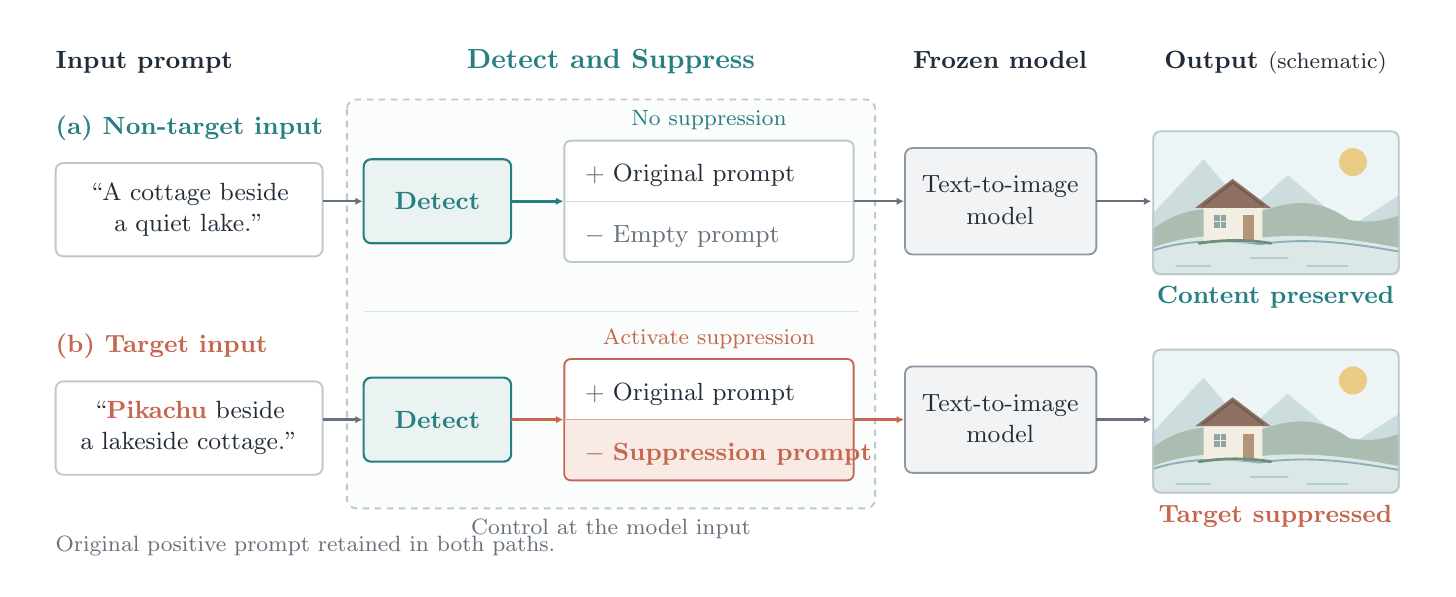
\begin{tikzpicture}[x=.336bp,y=-.336bp]
  \path[use as bounding box] (0,0) rectangle (1500,580);
  \fill[white] (0,0) rectangle (1500,580);

  \node[header] at (30,44) {Input prompt};
  \node[header,anchor=base,text=teal,font=\fontsize{10.08}{12.1}\selectfont\bfseries] at (625,44) {Detect and Suppress};
  \node[header,anchor=base] at (1042,44) {Frozen model};
  \node[header,anchor=base] at (1337,44) {Output {\normalfont\fontsize{7.73}{9.3}\selectfont (schematic)}};

  \draw[draw=edge,fill=panel,line width=.67pt,rounded corners=3.36pt,dash pattern=on 2.35pt off 2.02pt]
    (342,77) rectangle (908,515);
  \draw[edge!55,line width=.57pt] (360,304)--(890,304);

  % (a) A non-target input retains the empty negative prompt.
  \node[label,text=teal,font=\fontsize{9.07}{10.8}\selectfont\bfseries] at (30,114) {(a) Non-target input};
  \draw[edge,fill=white,line width=.67pt,rounded corners=2.69pt] (30,145) rectangle (316,245);
  \node[centered] at (173,185) {``A cottage beside};
  \node[centered] at (173,218) {a quiet lake.''};
  \draw[flow] (316,186)--(359,186);

  \draw[teal,fill=paleteal,line width=.77pt,rounded corners=2.69pt] (360,141) rectangle (518,231);
  \node[centered,text=teal,font=\fontsize{9.07}{10.8}\selectfont\bfseries] at (439,195) {Detect};
  \draw[detectflow] (518,186)--(574,186);
  \node[secondary,anchor=base,text=teal] at (730,105) {No suppression};

  \draw[edge,fill=white,line width=.67pt,rounded corners=2.35pt] (575,121) rectangle (885,251);
  \draw[edge!70,line width=.54pt] (575,186)--(885,186);
  \node[label,text=muted] at (597,165) {$+$};
  \node[label] at (627,165) {Original prompt};
  \node[label,text=muted] at (597,230) {$-$};
  \node[label,text=muted] at (627,230) {Empty prompt};
  \draw[flow] (885,186)--(939,186);

  \draw[modeledge,fill=modelbg,line width=.67pt,rounded corners=2.69pt] (940,129) rectangle (1145,243);
  \node[centered] at (1042,177) {Text-to-image};
  \node[centered] at (1042,211) {model};
  \draw[flow] (1145,186)--(1204,186);
  \pic at (1205,110) {landscape};
  \node[centered,text=teal,font=\fontsize{9.07}{10.8}\selectfont\bfseries] at (1337,296) {Content preserved};

  % (b) A detected target activates its paired suppression prompt.
  \node[label,text=coral,font=\fontsize{9.07}{10.8}\selectfont\bfseries] at (30,348) {(b) Target input};
  \draw[edge,fill=white,line width=.67pt,rounded corners=2.69pt] (30,379) rectangle (316,479);
  \node[centered] at (173,419) {``\textcolor{coral}{\textbf{Pikachu}} beside};
  \node[centered] at (173,452) {a lakeside cottage.''};
  \draw[flow] (316,420)--(359,420);

  \draw[teal,fill=paleteal,line width=.77pt,rounded corners=2.69pt] (360,375) rectangle (518,465);
  \node[centered,text=teal,font=\fontsize{9.07}{10.8}\selectfont\bfseries] at (439,429) {Detect};
  \draw[suppressflow] (518,420)--(574,420);
  \node[secondary,anchor=base,text=coral] at (730,339) {Activate suppression};

  \draw[coral,fill=white,line width=.67pt,rounded corners=2.35pt] (575,355) rectangle (885,485);
  \begin{scope}
    \clip[rounded corners=2.35pt] (576,356) rectangle (884,484);
    \fill[palecoral] (576,420) rectangle (884,484);
  \end{scope}
  \draw[coral!55,line width=.54pt] (575,420)--(885,420);
  \node[label,text=muted] at (597,399) {$+$};
  \node[label] at (627,399) {Original prompt};
  \node[label,text=coral] at (597,464) {$-$};
  \node[label,text=coral,font=\fontsize{9.07}{10.8}\selectfont\bfseries] at (627,464) {Suppression prompt};
  \draw[suppressflow] (885,420)--(939,420);

  \draw[modeledge,fill=modelbg,line width=.67pt,rounded corners=2.69pt] (940,363) rectangle (1145,477);
  \node[centered] at (1042,411) {Text-to-image};
  \node[centered] at (1042,445) {model};
  \draw[flow] (1145,420)--(1204,420);
  \pic at (1205,344) {landscape};
  \node[centered,text=coral,font=\fontsize{9.07}{10.8}\selectfont\bfseries] at (1337,530) {Target suppressed};

  \node[secondary] at (30,561) {Original positive prompt retained in both paths.};
  \node[secondary,anchor=base] at (625,543) {Control at the model input};
\end{tikzpicture}
\end{document}
